\chapter{Concepte Teoretice}

\section{Rețele neuronale}
\label{ANN}

Rețelele neuronale stau la baza tuturor algoritmilor moderni de inteligență artificială. Acestea au revoluționat industria învățării automate prin puterea lor de a simula funcțiile cognitive ale creierului uman, fiind des folosite în învățarea de tipare(în engleză pattern recognition), diferite sarcini de clasificare si predicție. Ele pot fi văzute ca funcții complicate care primesc date de intrare sub forma unor valori numerice și returnează valori reprezentative pentru acestea. 

\subsection{O scurtă istorie a rețelelor neuronale}

\begin{itemize}
    \item În lucrarea intitulată „A Logical Calculus of the Ideas Immanent in Nervous Activity”(1943) \cite{mcculloch1943logical} Warren McCulloch și Walter Pitts au fost primii care au teoretizat o implementare matematică simplificată a neuronului ca o poartă logică binară. Aceștia au demonstrat teoretic faptul că neuronii au capacitatea de a reprezenta orice funcție matematică.

    \item În 1958, este publicată lucrarea cercetătorului Frank Rosenblatt „The Perceptron: A Probabilistic Model for Information Storage and Organization in the Brain” \cite{rosenblatt1958perceptron}, în care acesta introduce conceptul de Perceptron, cel mai simplu model de rețea neuronală. 

    \newpage
    
    \item Spre finalul anilor 1980, după o lungă perioadă în care studiul rețelelor neuronale a fost neglijat, David E. Rumelhart, Geoffrey Hinton, and Ronald J. Williams (1986) \cite{rumelhart1986learning} prezintă \textbf{backpropagarea}, un algoritm prin care o rețea neuronală putea să învețe eficient, adresând multe dintre problemele ridicate până la acel moment. 

    \item La începutul anilor 2000, tot Geoffrey Hinton, de data aceasta alături de Ruslan Salakhutdinov \cite{hinton2006reducing} aduc o soluție pentru problema gradienților care dispar, prin reducerea dimensionalității datelor.
\end{itemize}

Aceste lucrări din literatură au ajutat la transformarea unor concepte pur teoretice în unelte cu putere de învățare și de decizie care au ajutat la modelarea industriei moderne și au împins progresul tehnologic către noi limite. 

\subsection{De la neuronul biologic la cel artificial}
    La fel ca multe dintre invențiile revoluționare de-alungul istoriei, cercetătorii au avut ca sursă de insipirație viețuitoarele. În cazul inteligenței artificiale, aspirația cercetătorilor a fost să replice neuronul biologic. 
    
    \begin{figure}[h]
         \centering 
         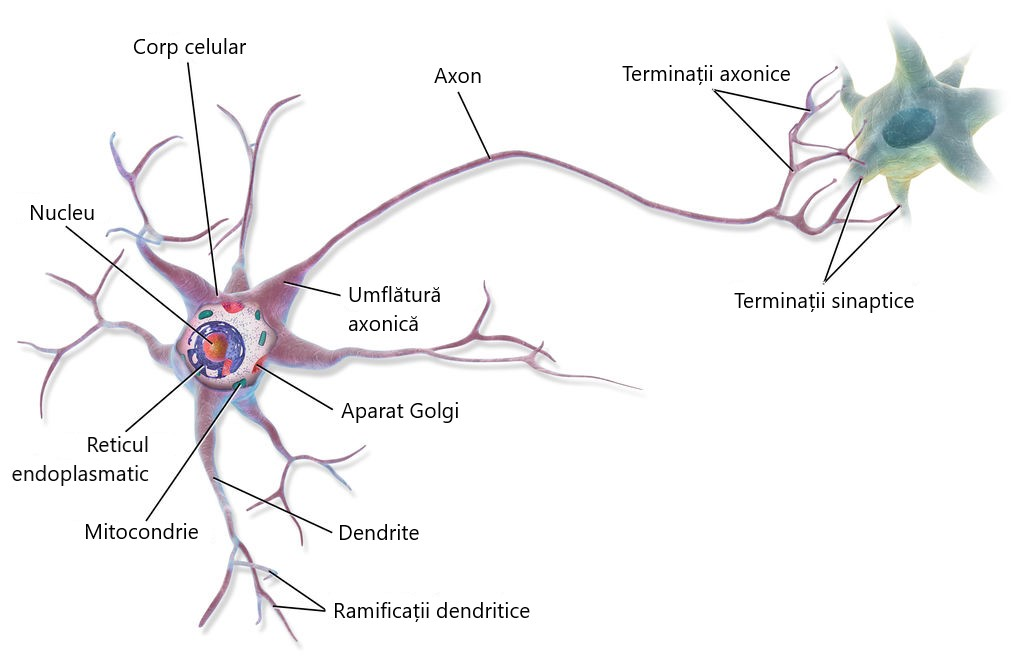
\includegraphics[width=.75\textwidth]{images/structura-unui-neuron.jpg}
         \caption{Anatomia unui neuron \cite{neuron-anatomy}}
    \end{figure}
    
    În zona centrală a neuronului se află corpul celular(soma) care conține nucleul, locul care înmagazineaza tot materialul genetic al celulei. Legate de corpul celular sunt dendritele, care interceptează semnale chimice de la alți neuroni. Atașat de corpul celular, se află o prelungire alungită numită axon, al cărei scop este să transmită semnale electrice către alți neuroni sau către țesuturi. La capătul axonului se găsesc terminațiile acestuia, care sunt legate de dendritele sau de corpul celular ale altui neuron. 

    În creierul biologic, se găsesc miliarde de neuroni, fiecare având mii de legaturi cu alți neuroni aceștia fiind dipusi in straturi pentru a crea țestul nervos. Cu toate că neuronul in sine, nu funcționează intr-un mod complex, ansamblul a miliarde de mecanisme simple într-o rețea imensa are capabilități impresionante. 

    Plecând de la aceste premise Warren McCulloch și Walter Pitts(1943) 
    \cite{mcculloch1943logical} au prezentat în lucrarea lor revoluționară o versiune simplificată a neuronului biologic. Aceștia au văzut neuronul artificial ca o pe poartă logică, cu mai multe intrări și o singură ieșire. Un semnal electric era transmis mai departe doar dacă neuronul avea un număr de intrări care trecea de un anumit prag, bazându-se pe principiul de totul sau nimic al neuronilor biologici.  

     \begin{figure}[h]
         \centering 
         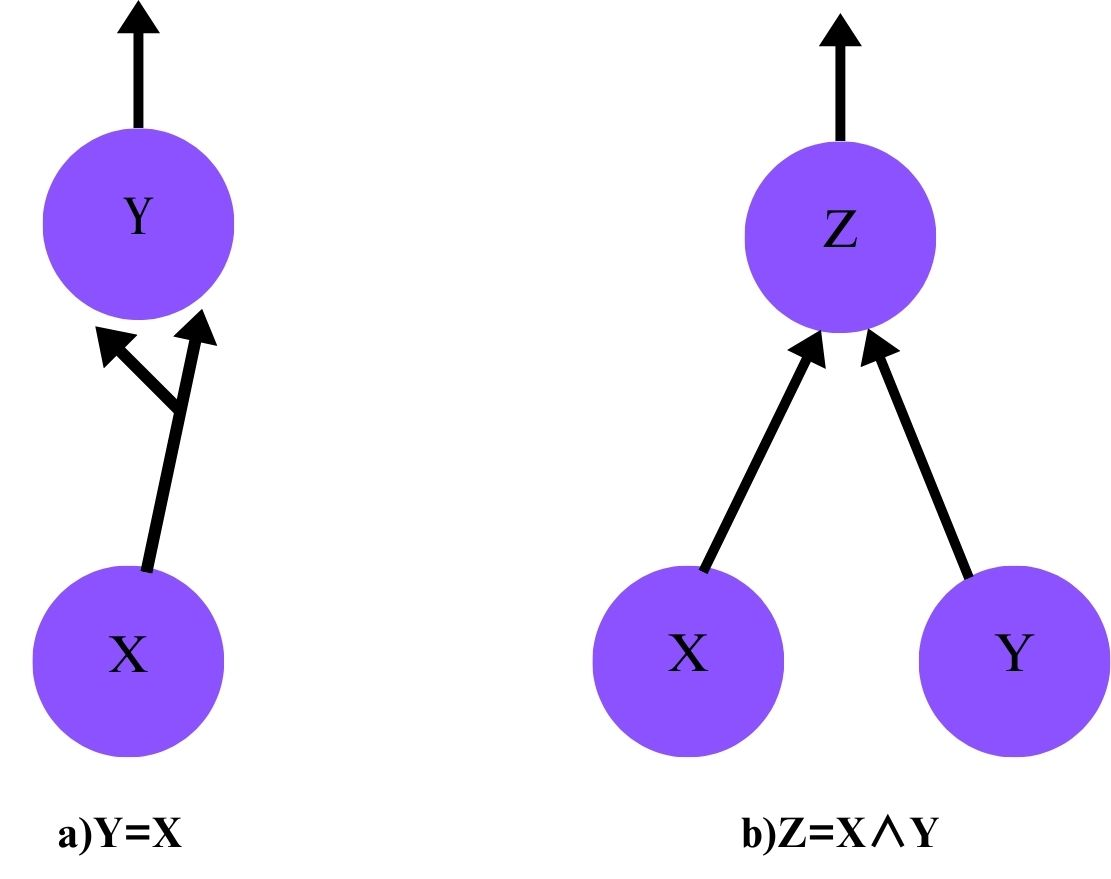
\includegraphics[width=.5\textwidth]{images/artificial-neurons-as-logic-gates.jpg}
         \captionsetup{font=footnotesize}
         \caption{Neuroni artificiali calculând operatii logice}
         \caption*{a) Neuronul Y nu poate transmite semnalul mai departe              doar cu un singur impuls}
         \caption*{b) Neuronul Z are nevoie de ambii neuroni X și Y pentru a trimite un semnal mai departe}
    \end{figure}

    \newpage

\subsection{Perceptronul}
\label{ch: Perceptron}
În 1958 Frank Rosenblatt \cite{rosenblatt1958perceptron} introduce in literatură \textbf{perceptronul}, cel mai simplu model de rețea neuronală. Acesta duce neuronul artificial propus de către McCulloch și Pitts \cite{mcculloch1943logical} la un alt nivel. Comparat cu neuronul care transmitea doar semnale binare, cel propus de Rosenblatt este capabil sa proceseze și să transmită mai departe valori numerice. Scopul final este de a organiza aceste unități de calcul într-o „rețea” care primește datele de intrare sub formă numerică și returnează o valoare care le reprezintă. 

Într-o astfel de rețea fiecare neuron se folosește datele de intrare pentru a produce o valoare de ieșire. Fiecărei valori de intrare îi corespunde o \textbf{pondere}(în engleză: weight), un număr real al cărui scop este sa controleze contribuția sa la informația transmisă mai departe de către neuron. Aceste valori sunt însumate ponderat, iar la valoarea obținută se adaugă un parametru special, numit \textbf{bias}, un număr real, notat cu $b$, care elimină constângerea ca funcția ce reprezintă datele să treacă prin originea planului sau a hiperplanului. Rezultatul reprezintă o funcție care este dată ca parametru unei funcții liniare numită „funcție de pas”(in engleză: step function) pentru a produce valoarea de ieșire a perceptronului. 

\begin{figure}[h]
         \centering 
         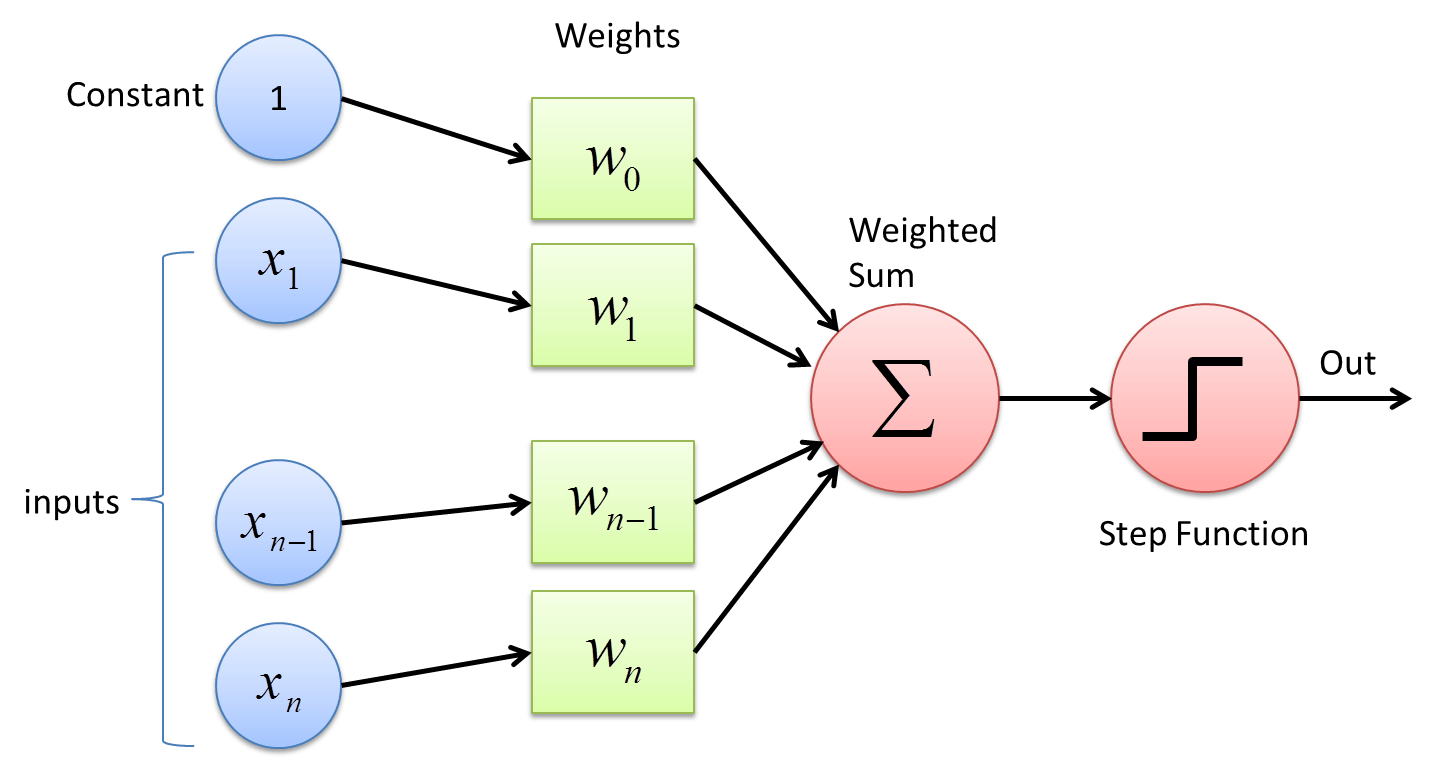
\includegraphics[width=.85\textwidth]{images/the-perceptron.jpg}
         \captionsetup{font=footnotesize}
         \caption{Perceptronul \cite{the-perecptron}}
\end{figure}
\newpage
Notații:

\begin{itemize}
    \item $x = (x_1, x_2, x_3... , x_n)$ : datele de intrare
    \item $w = (w_1, w_2, w_3,..., w_n)$ : ponderile corespunzătoare 
    \item $b$ : multimea paremtrilor de tip \textit{bias} 
    \item $z$ : combinația liniară dintre $x$ și $w$
    \item $z = w_1 x_1 + w_2 x_2 + ... + w_n x_n  = \sum_{i=1}^{n} w_i x_i + b = w^{T}x + b$
    \item $step(z)$ : \textit{output-ul} unității de calcul
\end{itemize}
 
O funcție comună folosită drept \textit{step function} este funcția semn definită astfel: 

\[
\text{sgn}(x) = 
\begin{cases} 
    -1 & \text{if } x < 0, \\
    0 & \text{if } x = 0, \\
    1 & \text{if } x > 0.
\end{cases}
\]    

\begin{figure}[h]
         \centering 
         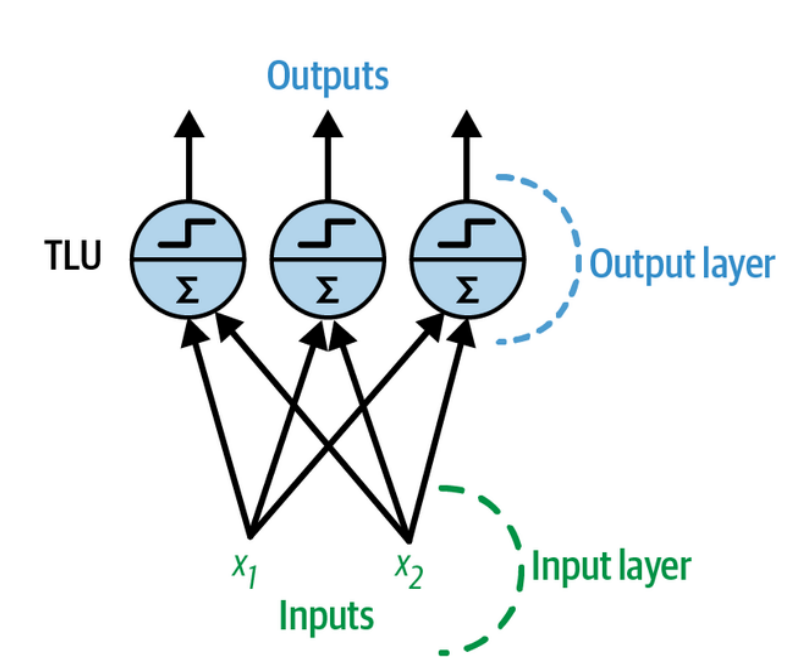
\includegraphics[width=.5\linewidth]{images/multiclass-perceptron.png}
         \captionsetup{font=footnotesize}
         \caption{Un perceptron capabil să separe date în mai multe clase \cite{ageron2019}}
         \label{Figura 2.4}
\end{figure}
\newpage

În Figura~\ref{Figura 2.4} este prezentată o arhitectură de perceptron capabilă sa distingă între 3 clase. Datele de intrare, in cazul nostru $x1$, $x2$ reprezintă \textit{stratul de intrare}. Fiecare valoare din stratul de intrare este legată de toți neuronii din stratul urmator, fiecare legatură având o pondere individuală. Stratul care produce valorile de ieșire se numește \textit{stratul de ieșire} și in exemplul prezentat este format din 3 neuroni, corespunzători fiecărei clasificări posibile. 

În ciuda optimismului declanșat de capabilitățile remarcabile la acea vreme a perceptronului, în 1969 Marvin Minsky și Seymour Papert \cite{minsky1969introduction} au demonstrat limitarea acestui model de a rezolva cateva probleme triviale, precum operația XOR. 

\subsection{Multilayer Perceptron(MLP)}

Soluția pentru limitările perceptronului a fost publicată de David Rumelhart, Geoffrey Hinton și Ronald Williams(1986) \cite{rumelhart1986learning}. Rezolvarea acestor probleme a constituit unificarea mai multor rețele de tip perceptron intr-o rețea mai mare, numită Multilayer Perceptron(MLP).


\begin{figure}[h]
         \centering 
         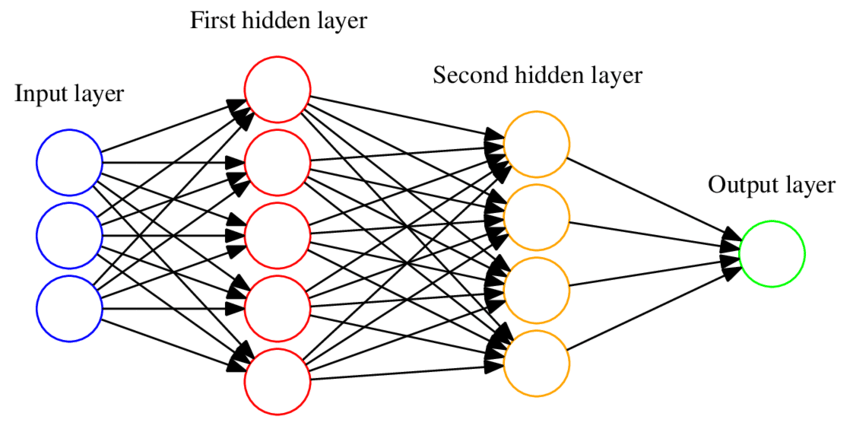
\includegraphics[width=.6\linewidth]{images/MLP.png}
         \captionsetup{font=footnotesize}
         \caption{Arhitectura de tip MLP(Multilayer Perceptron) \cite{phdthesis}}
\end{figure}

\begin{itemize}
    \item Stratul de input(\textbf{input layer}) = stratul ce conține doar valorile de intrare
    \item Straturile ascunse(\textbf{hidden layers} = straturile prin care se propaga informația. Se sitează între stratul de input și cel de output
    \item Stratul de output(\textbf{output layer}) = stratul care ne oferă rezultatul trecerii informației prin rețea
\end{itemize}

% \newpage
Arhitectura MLP este una de tip \textbf{feedforward}, cu alte cuvinte, informația se propagă prin rețea intr-o singură direcție, de la stânga la dreapta(dinspre input către output), în care toate straturile sunt \textbf{fully connected}, fiecare unitate de calcul este conectată de toți neuronii din următorul strat. 

În lucrarea lor, cercetătorii au arătat ca rețeaua poate să învețe informații relevante cu ajutorul algoritmului de \textbf{backpropagare}. 
\subsection{Backpropagarea}

Algoritmul prin care o rețea neuronală învață se numește \textbf{backpropagation}. Acesta presupune trecerea prin rețea în repetate rânduri, în doi pași(\textbf{forward pass}): unul inainte și unul înapoi(\textbf{backward pass}). Dupa fiecare trecere parametrii(ponderile) sunt actualizați pentru a obține predicții mai bune.
Algoritmul poate fi descris astfel:
\begin{itemize}
    \item Setul de date este spart în blocuri mai mici, cele mai întâlnite dimensiuni fiind de 32, 64 sau 128 de instanțe per bloc
    \item Fiecare bloc este trecut prin rețea: se calculează output-ul primului strat, care este dat ca intrare pentru urmatorul strat, continuând în același fel până se ajunge la stratul de output. Acesta reprezintă \textbf{forward pass-ul}.
    \item Se evaluează performanța predicțiilor cu ajutorul unei funcții numită \textbf{funcție de pierdere}. Scopul acestei funcții este să furnizeze un scor care să descrie cât de precise au fost predicțiile rețelei față de rezultatul dorit. 
    \item Dupa calculul erorii, algoritmul calculează contribuția fiecărei ponderi din rețea la eroarea totală, cu ajutorul regulii fundamentale din analiza matematică: regula înlănțuirii(în engleză: \textit{chain rule}).
    \item Contribuția la eroarea totală a unui parametru se numește \textbf{gradient}.Valoarea gradientului unui parametru practic măsoară cât de mult influențează eroarea totală modificarea acestuia.
    \item În cele din urmă, algoritmul folosește gradienții calculați pentru a modifica parametrii cu ajutorul \textbf{algoritmului coborârii pe gradient}.
\end{itemize}
\newpage


\subsection{Algoritmul coborârii pe gradient(\textit{Gradient Descent})}
\label{ch:Gradient Descent}
Coborârea pe gradient este un algoritm iterativ de optimizare, folosit des în literatură, al cărui scop este de găsi minimul global al unei funcții. În cadrul rețelelor neuronale acesta este folosit pentru a optimiza parametrii rețelei astfel încat valoarea erorii totale să se apropie la fiecare iterație de minimul funcției de pierdere. Dupa calcularea gradienților, fiecare pondere se actualizeaza după formula: 
\begin{equation}
    \scalebox{1.2}{$w_{\text new} = w - \eta \frac{\delta L}{\delta w}$}
    \label{}
\end{equation}

Unde: 

\begin{itemize}
    \item $w_{\text new}$ : noua valoare a ponderii
    \item $L$ : valoarea funcției de pierdere
    \item $\frac{\delta L}{\delta w}$ : gradientul 
    \item $\eta$ : rata de învățare(hiperparametru ce controleaza cât de mult se modifică valorile ponderilor)
\end{itemize}

\begin{figure}[h]
         \centering 
         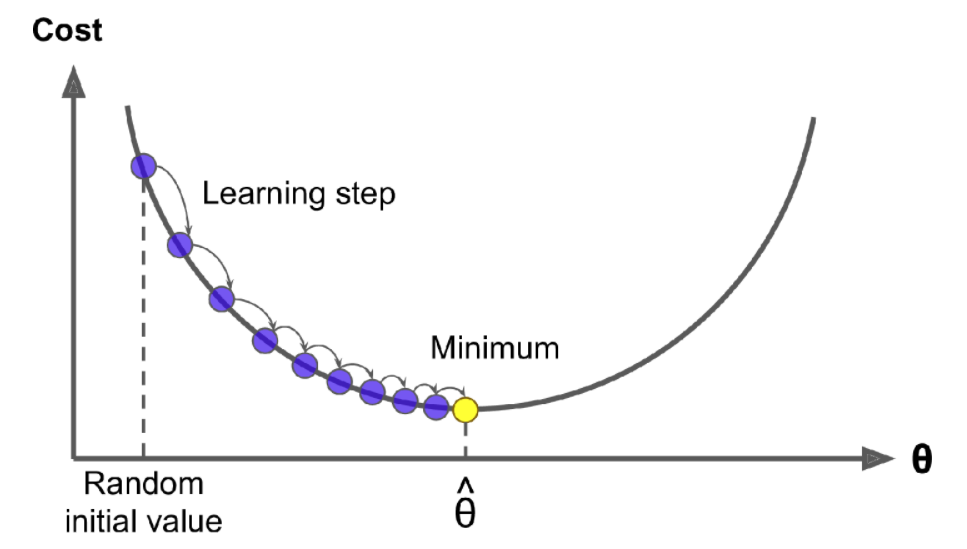
\includegraphics[width=.75\linewidth]{images/gradient-descent.png}
         \captionsetup{font=footnotesize}
         \caption{Vizualizare a algoritmului de coborârii pe gradient \cite{GD}}
\end{figure}
\newpage
Pentru a folosi algoritmul coborârii pe gradient în cadrul backpropagării Rumelhart et al. au înlocuit în aceeași lucrare \cite{rumelhart1986learning} funcția de pas(step function) cu funcția logistică(numită și sigmoidă).
\begin{equation}
    \scalebox{1.2}{$\sigma(x) = \frac{1}{1 + e^{-x}}$}
    \label{eq: Funcția sigmoidă}
\end{equation}
În urma modificării, denumirea de funcție de pas a fost înlocuită cu termenul de \textbf{funcție de activare}. Funcția logistică nu este singura funcție de activare care oferă rezultate în practică. Alte opțiuni des întâlnite în literatură pentru \textbf{straturile ascunse} sunt: 
\begin{itemize}

    \item \textbf{Tangenta hiperbolică}:
    \begin{equation}
        \tanh(x) = \frac{e^x - e^{-x}}{e^x + e^{-x}}
        \label{}
    \end {equation}
    
    \item \textbf{ReLU(Rectified Linear Unit)}:
    \begin{equation}
    \text{ReLU}(x) = 
        \begin{cases} 
        0 & \text{if } x \leq 0 \\
        x & \text{if } x > 0 
        \end{cases}
        \label{}
    \end {equation}
        
    \item \textbf{Leaky ReLU}:
    \begin{equation}
    \text{Leaky ReLU}(x) = 
        \begin{cases} 
        \alpha x & \text{if } x < 0 \\
        x & \text{if } x \geq 0 
        \end{cases}
        \label{}
    \end {equation}
    
\end{itemize}

Aspectul ce diferențiază funcțiile de activare față de funcțiile de pas, sunt 2 proprietăți esențiale:

\begin{itemize}
    \item \textbf{Sunt diferențiabile în orice punct}: acest lucru face posibilă calcularea gradienților și folosirea algoritmilor de optimizare.
    \item \textbf{Sunt nelineare}, ceea ce contribuie decisiv la capacitatea modelelor de a surprinde si învăța informații mult mai complexe din datele de antrenare.  
\end{itemize}



\newpage

\begin{figure}[h]
         \centering 
         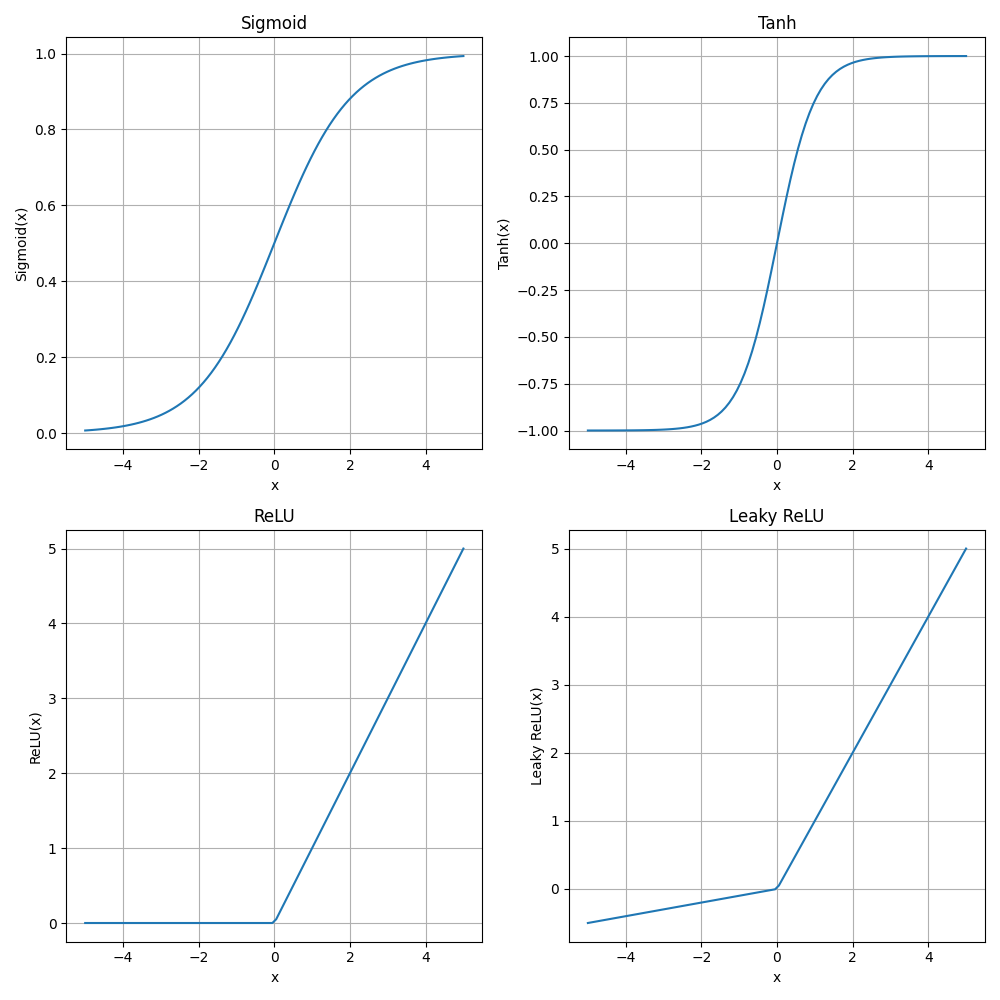
\includegraphics[width=.6\linewidth]{images/activation_functions.png}
         \captionsetup{font=footnotesize}
         \caption{Funcții de activare}
\end{figure}

Funcțiile de activare prezentate anterior sunt folosite în straturile ascunse pentru a crea transfromări nelineare ale valorilor, cu scopul de a surprinde substraturi complexe ale datelor. 

Pentru stratul de ieșire, obiectivul este de a adapta funcția de activare pentru sarcina specifică a rețelei, fie că este o probabilitate, o clasă sau o valoare continuă. În literatură cele mai des întâlnite sunt: 

\begin{itemize}
    \item Pentru clasificarea binară se folosește funcția sigmoidă (ecuația \ref{eq: Funcția sigmoidă}). 
    \item Pentru task-uri de regresie(predicția unei valori continue) se folosește funcția identitate:
    \begin{equation}
        f(x) = x
        \label{}
    \end{equation}
    \item Pentru clasificare multiplă se folosește funcția \textbf{softmax} care este o generalizare a funcției sigmoide:
        \begin{equation}
        \sigma(\mathbf{z})_j = \frac{e^{z_j}}{\sum_{k=1}^K e^{z_k}}
        \label{}
    \end{equation}
\end{itemize}


\begin{figure}[h]
         \centering 
         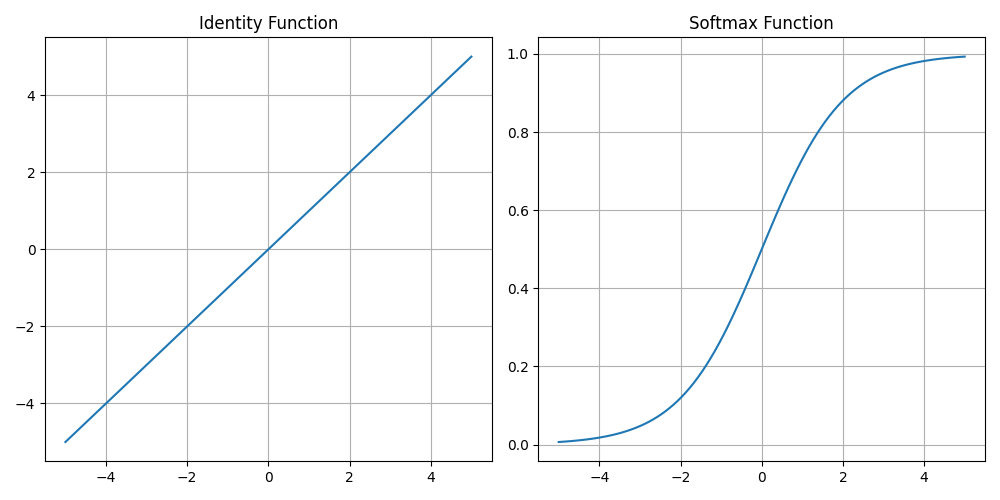
\includegraphics[width=.65\linewidth]{images/activation_functions_output.png}
         \captionsetup{font=footnotesize}
         \caption{Funcția idenitate și funcția softmax}
         \label{}
\end{figure}


\subsection{Optimizarea în practică și alți algoritmi de optimizare}

Antrenarea rețelelor neuronale este laborioasă și consumatoare de timp, mai ales pentru seturi voluminoase de date. De aceea, aceasta necesită valori cât mai apropiate de optim pentru hiperparametri, deoarece aceștia controlează antrenarea. 

Un pas important în optimizarea timpului de antrenare este alegerea unei rate de învățare potrivită. O rată de învățare optimă, ajută la reducerea timpului de convergență către optimul global. 

\begin{figure}[h]
         \centering 
         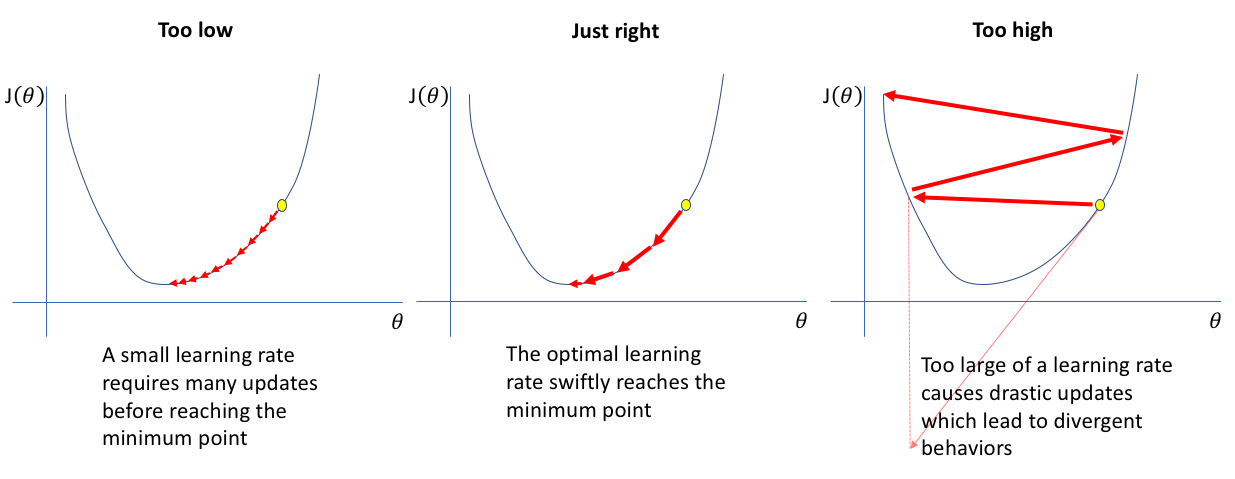
\includegraphics[width=.85\linewidth]{images/learning_rate.png}
         \captionsetup{font=footnotesize}
         \caption{Rata de învățare afectează convergența\cite{learning-rate}}
         \label{Figura 2.9}
\end{figure}
În prima imagine din figura \ref{Figura 2.9} se poate observa că o valoare prea mică necesită mai mulți pași pentru a ajunge la convergență. De asemenea, o rată de învățare mică poate determina blocajul într-un minim local. 

În a treia imagine este folosită o rată de invățare prea mare, ceea ce determină divergență(îndepărtarea de minimul global). 

În cea de-a doua imagine pașii sunt mai mari la inceput, iar pe măsură ce pierderea se apropie de minim, pașii devin tot mai mici.

Metodele utilizate în practică încearcă să îmbunătățească timpul de convergență prin diferite procedee matematice, ce implică mai multi parametri decât rata de învățare. Un exemplu robust și foarte des întâlnit este algoritmul coborârii pe gradient varianta stocastică(abreviat \textbf{SGD}, din denumirea în engleză \textbf{Stochastic Gradient Descent}) cu momentum. 

Spre deosebire de algoritmul clasic care folosește tot setul de date pentru a face o actualizare a ponderilor in rețea, varianta stocastica a acestuia alege subseturi alese aleator ceea ce îmbunătațește considerabil convergența. 

Pentru a crește performanța și mai mult, Boris T. Polyak\cite{polyak1964some} a introdus în 1964 \textbf{momentumul}. Fenomenul de momentum poate fi comparat cu rostogolirea unui bulgăre de zăpadă, care pe măsură ce se deplasează își mărește dimensiunea și se mișcă din ce în ce mai repede. 

În practică, această acumulare de valori este implementată cu ajutorul unui vector(notat cu $v$) care funcționează ca o „memorie” ce folosește gradienții anteriori pentru a face coborârea pe gradient mai „lină” și pentru a evita eventualele blocaje în puncte de minim locale. Acesta este inițializat cu 0 si la fiecare pas este actualizat în funcție de valoarea anterioară ($v_{t-1})$ și de valoarea gradientului funcței de pierdere, dupa formula:

\begin{equation}
    v_t = \beta v_{t-1} + (1 - \beta) \nabla_{\theta} J(\theta)
\end{equation}

Apoi ponderile sunt actualizate folosind vectorul $v_t$

\begin{equation}
    \theta = \theta - \eta v_t
\end{equation}

\newpage

Notații:

\begin{itemize}
    \item $v_t$ : vectorul $v$ la momentul t
    \item $\beta$ : coeficientul pentru momentum
    \item $\nabla_{\theta} J(\theta)$ : gradientul funcției de pierdere $J$, în raport cu paremtrii $\theta$ calculați la pasul curent
    \item $\eta$ : rata de învățare
\end{itemize}

SGD cu momentum este doar unul din multe alte metode optimizare. În literatură sunt sunt des întâlniți și:

\begin{itemize}
    \item \textbf{AdaGrad}\cite{duchi2011adaptive}: face actualizări mai mari pentru exemplele rare și actualizări mai mici pentru cele întâlnite mai des. 
    \item \textbf{RMSprop}\cite{rmsprop} folosește declin exponențial(exponential decay) pentru gradienții vechi pentru a diminua influența acestora. 
    \item \textbf{Adam}\cite{kingma2014adam}, se folosește atât de proprietățile algoritmului AdaGrad, dar și de cele ale lui RMSprop.
\end{itemize}

\subsection{Overfitting vs underfitting}

O problemă cu care se confruntă rețelele neuronale este faptul că sunt influențate prea mult de datele cu care sunt antrenate, iar acest lucru le afectează performanța atunci cand sunt expuse la exemple noi. Acest fenomen se numește \textbf{overfitting} și în general este caracterizat de diferențe mari între performanța predicțiilor pe datele de antrenare și cele de testare. Cauze comune pentru overfitting:

\begin{itemize}
    \item \textbf{Modele prea complexe}: Modelele cu un număr mare de parametri pot să fie modelate la perfecție pe datele de antrenare, încluzând zgomotul
    \item \textbf{Date insfuciente}: Seturile de date prea mici fac modelul să învețe datele, în locul unor metode de învățare generale.
\end{itemize}

Soluții comune pentru overfitting sunt metode precum: \textbf{dropout}\cite{srivastava2014dropout}, \textbf{regularizare L1, L2} \cite{ng2004feature} sau \textbf{cross-validation} \cite{kohavi1995study}

Problema de la polul opus se numește \textbf{underfitting}, caracterizat de performanțe slabe ale modelului atât pe setul de antrenare cât și pe cel de testare. Probleme des întâlnite: complexitate insufcientă a modelului, antrenare insuficientă, regularizare prea mare sau date de calitate prea slabă.
Soluțiile sunt de cele mai multe ori rezolvarea problemelor menționate anterior.

\begin{figure}[h]
         \centering 
         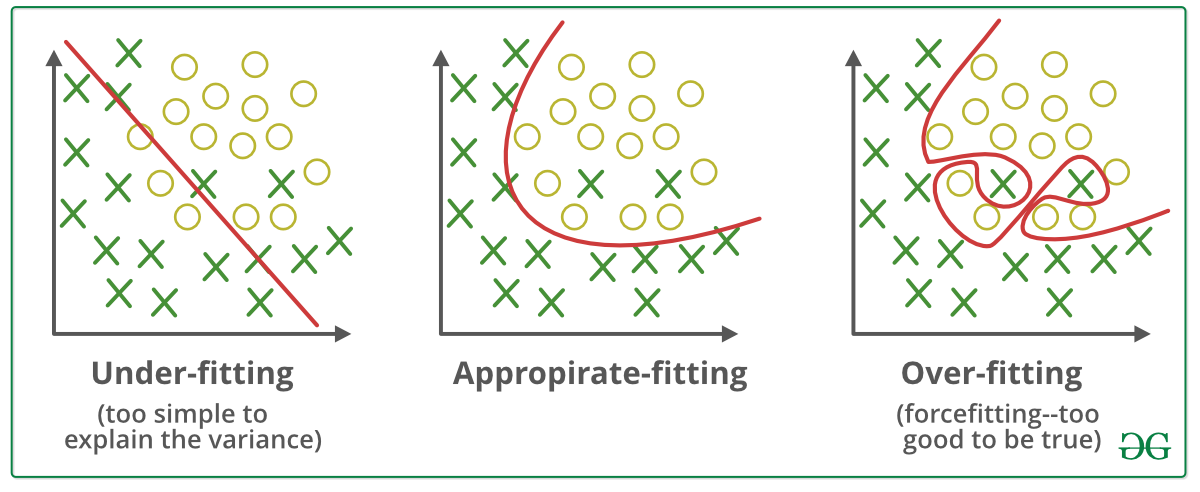
\includegraphics[width=.85\linewidth]{images/under_vs_over.png}
         \captionsetup{font=footnotesize}
         \caption{Overfitting vs underfitting \cite{under_vs_over}}
\end{figure}


\newpage



\section{Rețele Neuronale Convoluționale}

Rețelele neuronale convoluționale(abreviate CNN, din engelză \textit{Convolutional Neural Networks)} au reprezentat un salt monumental în domeniul învățării adânci(Deep Learning), redefinind limitele puterii de învățare a rețelelor neuronale. 

În capitolul \ref{ANN} au fost prezentate conceptele fundamentale din spatele rețelelor neuronale, urmând ca în acest capitol să fie discutat un tip de rețea specializată pe procesarea imaginilor.
Rețelele convoluționale diferă față de cele tradiționale prin structura și funcționalitatea lor unică, proiectată pentru detecția și învățarea trăsăturilor repetitive din date, în special din imagini.

Obiectivul rețelelor convoluționale este de a replica un proces din cortexul creierului uman, unde anumiți neuroni sunt specializați pentru a observa diverse detalii din câmpul vizual. Acest proces biologic este implementat folosind \textbf{straturi convoluționale}. 

Spre deosebire de MLP-uri, rețelele convoluționale nu folosesc straturi fully connected, ci straturi convoluționale care folosesc filtre învățabile pentru a extrage detalii din date. Această abordare încurajeaza utilizarea rețelelor cât mai adânci deoarece straturile convoluționale folosesc un număr semnificativ mai mic de parametri.

\subsection{Rețelele convoluționale de-alungul anilor}

\begin{itemize}
    \item \textbf{LeNet-5(1998)}\cite{lecun1998gradient}: În 1998 Yann Lecun et al. prezintă ceea ce este considerat de mulți prima implementare practică a rețelelor convoluționale. Lucrarea lor a prezentat lumii capabilitățile acestui tip de rețea în proceseara imaginilor, folosindu-se de datasetul \href{https://en.wikipedia.org/wiki/MNIST_database}{MNIST}.

    \item \textbf{ImageNet și AlexNet(2012)}\cite{krizhevsky2012imagenet}: \href{https://en.wikipedia.org/wiki/ImageNet}{ImageNet} este o baza de date ce conține aproximativ 14 milioane de imagini din peste 20000 de categorii. Aceasta a fost pusă la dispoziție in 2010, dând start competiției cu același nume, devenind etalonul de performanță pentru vederea artificială. În anul 2012 arhitectura AlexNet, proiectată de Alex Krizhevsky, Ilya Sutskever și Geoffrey Hinton, a câștigat detașat competiția folosind o rețea antrenată în premieră pe doua plăci grafice. 

    \item \textbf{VGG, GoogLeNet și ResNet(2014-2015)}\cite{simonyan2014very, szegedy2015going, he2016deep}: VGG-16 si VGG-19 sunt arhitecturi care au demonstrat importanța adâncimii în rețelele convoluționale. GoogleNet, numită și Inception-v1 a introdus convoluțiile mixte, în timp ce ResNet a dus performanțele rețelelor convoluționale la alt nivel cu ajutorul legăturilor reziduale.
\end{itemize}

\subsection{Straturile convoluționale}

Piesa de bază a rețelelor convoluționale este operația de \textbf{convoluție}. Această operație folosește un filtru (o matrice, de obicei pătratică), care este glisat peste o altă matrice(o imagine, în acest caz particular) și efectueaza înmulțiri și adunări pentru a surprinde detalii precum muchii sau texturi. Rezultatele convoluțiilor se numesc hărți de trăsături(\textbf{feature maps}). 

Fie \(X\) matricea imaginii de intrare sau o hartă de trăsături dintr-un strat precedent, unde \(X\) este de dimensiune \(M \times N\) (M linii și N coloane).
Fie \(K\) un filtru de dimensiune \(a \times b\) (a linii și b coloane).

Operația de convoluție glisează filtrul\(K\) peste matricea \(X\), calculând produsul scalar dintre K și o porțiune de dimeniunea lui K din imagine. Rezultatul \(Y\) respectiv fiecărei poziții \((i, j)\) se calculeaza după formula:

\begin{equation}
    Y(i, j) = \sum_{u=0}^{a-1} \sum_{v=0}^{b-1} K(u, v) \times X(i+u, j+v)
    \label{2.10}
\end{equation}

În formula \ref{2.10}, \(u\) și \(v\) sunt indicii ce pargurg dimensiunile lui \(K\), în timp ce \((i+u, j+v)\) sunt coordonatele ce localizează bucata de imagine din \(X\) căreia urmează să îi fie aplicat filtrul. Figura \ref{Figura 2.10} oferă o vizualizare clară a operației de convoluție.

\begin{figure}[h]
         \centering 
         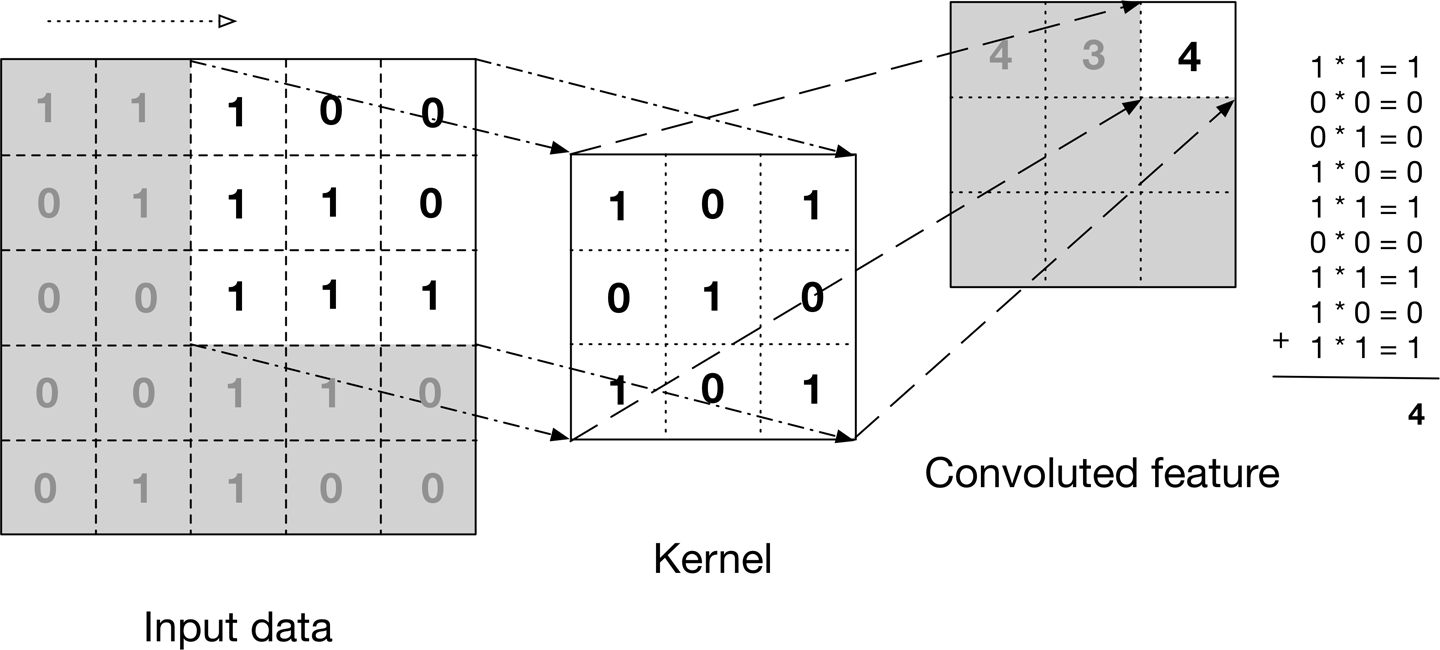
\includegraphics[width=.85\linewidth]{images/Convolutie.png}
         \captionsetup{font=footnotesize}
         \caption{Vizualizare a operației de convoluție\cite{convolution}}
         \label{Figura 2.10}
\end{figure}
\newpage
\subsection{Stride și padding}

Până acum operația de convoluție a fost făcută cu presupunerea că filtrul este deplasat la fiecare pas cu câte un pixel. Pasul făcut de către filtru în timpul convoluției se numește \textbf{stride}.
Pentru o matrice \(X\) de dimensiune \(M \times N\) și un filtru \(K\) de dimensiune \(a \times b\), dimensiunile hărții de trăsături pentru stride-ul $s$ vor fi:

\begin{equation}
    \begin{aligned}
        \text{Output\_height} &= \left\lfloor \frac{M - a}{s} \right\rfloor + 1 \\
        \text{Output\_width} &= \left\lfloor \frac{N - b}{s} \right\rfloor + 1
    \end{aligned}
    \label{stride}
\end{equation}
\\
\begin{figure}[h]
         \centering 
         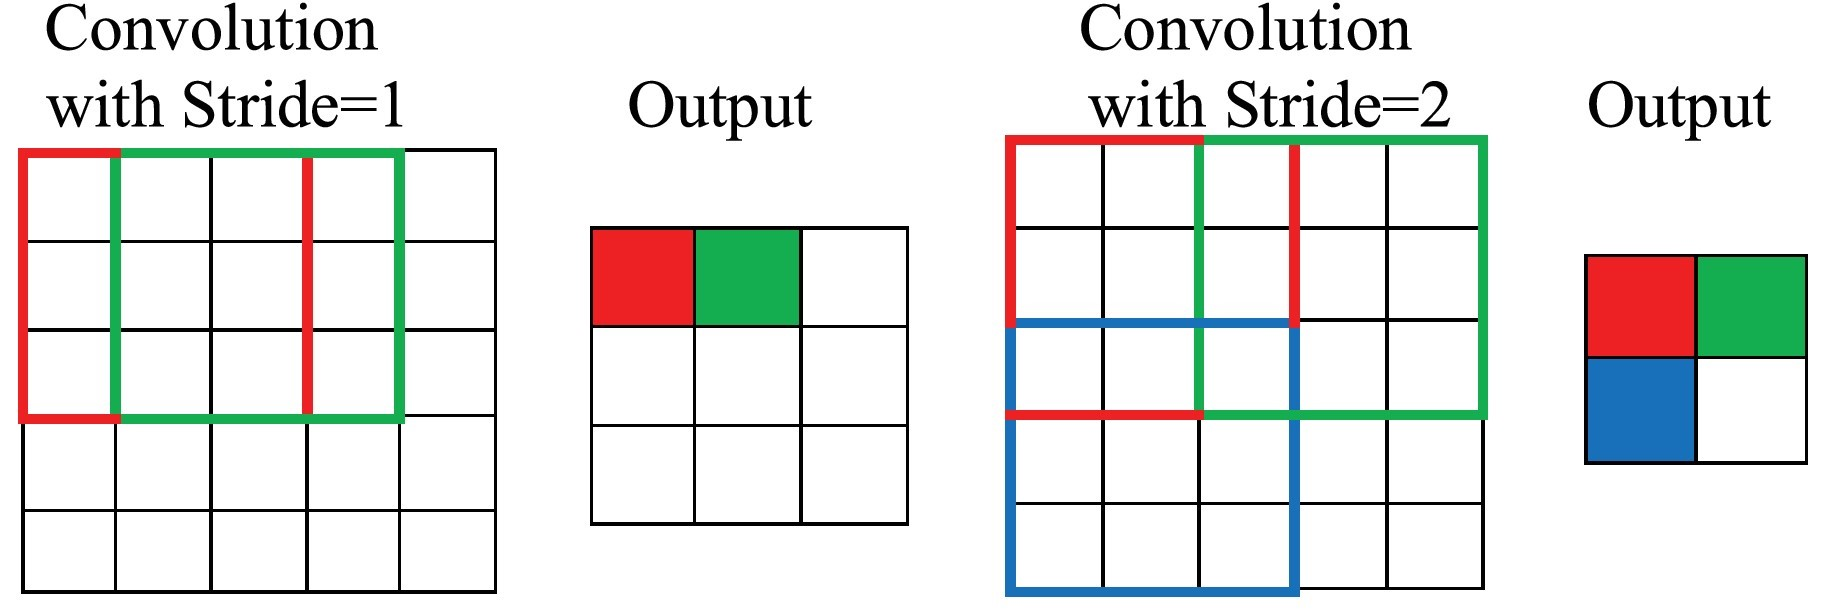
\includegraphics[width=0.85\linewidth]{images/stride.jpg}
         \captionsetup{font=footnotesize}
         \caption{Folosirea stride-ului reduce dimensiunea ieșirii\cite{stride}}
\end{figure}

Folosirea stride-ului în rețelele convoluționale are diverse scopuri:

\begin{itemize}
    \item \textbf{Reduce dimnensionalitatea și eficientizează antrenare}: Stride-ul reduce dimensiunea hărții de trăsături pe care o primește ca input. Acest lucru ajută la gestionarea complexității computaționale și la evitarea unor posibile probleme legate de memoria insuficientă și totodată îmbunătățește timpul de antrenare semnificativ.

    \item \textbf{Crește câmpul vizual}: Folosirea unei valori mai mari pentru stride ajută la capturararea trăsăturilor cu mai mult context global, deoarece output-ul corespunde unei regiuni mai mari din imaginea de input. 

    \item \textbf{Controlează suprapunerea filtrelor}: Cu valoarea stride-ului setată la 1, filtrele se suprapun semnficativ ceea ce poate duce la propagarea unor trăsături redundante. 
\end{itemize}

\textbf{Constrângeri ale valorii stride-ului}:

\begin{itemize}
    \item Dimensiunea pentru output trebuie să fie număr întreg:
        \begin{equation}
        \begin{aligned}
            \text{Output\_height} &= \left\lfloor \frac{M - a}{s} \right\rfloor + 1 \in \mathbb{Z} \\
            \text{Output\_width} &= \left\lfloor \frac{N - b}{s} \right\rfloor + 1 \in \mathbb{Z}
        \end{aligned}
        \label{}
        \end{equation}
    \item Compatibilitate cu \textbf{padding-ul}(hiparametru explicat mai jos) pentru a obține dimensiune dorită pentru output
\end{itemize}

Atunci când se folosesc multe convoluții consecutive, matricea de trăsături se micșorează semnificativ. \textbf{Padding-ul} este un procedeu folosit în rețelele convoluționale pentru a controla dimensiunile output-ului, ce presupune adăugarea de pixeli pe marginea matricei de intrare. Cu ajutorul lui putem obține o hartă de activare cu aceleași dimensiuni ca matricea de input. Padding-ul este de 2 tipuri:

\begin{itemize}
    \item \textbf{Valid}: micșorează output-ul:
        \begin{equation}
            \begin{aligned}
            \text{Output\_height} &= {M - a} + 1  \\
            \text{Output\_width} &= {N - b} + 1 
        \end{aligned}
        \end{equation}
    \item \textbf{Same}: păstrează dimensiunea intrării. Padding-ul necesar pentru un filtru pătratic este calculat după formula:

    \begin{equation}
        p = \frac{k-1}{2}
    \end{equation}

    Pentru $K$, un filtru de dimensiune $k\times k$
    
\end{itemize}

\begin{figure}[h]
         \centering 
         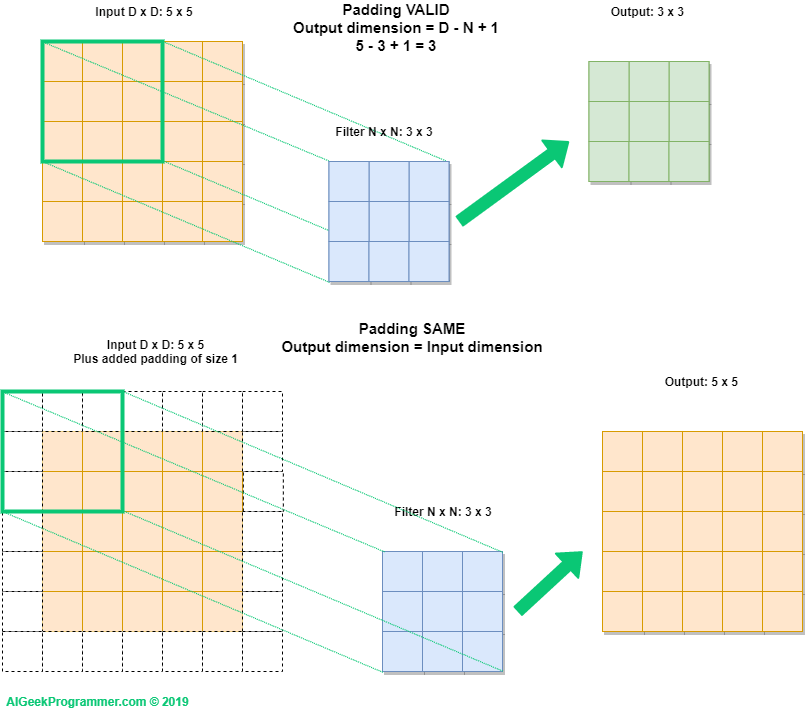
\includegraphics[width=0.75\linewidth]{images/padding.png}
         \captionsetup{font=footnotesize}
         \caption{Tipuri de padding\cite{padding}}
\end{figure}
În practică padding-ul este folosit alături de stride. Pentru a calcula valorile necesare, formulele anterioare se modifică:

\textbf{Dimensiunile output-ului în funcție de stride, padding și filtru}:

\begin{equation}
    \begin{aligned}
        \text{Output\_height} &= \left\lfloor \frac{M + 2p - a}{s} \right\rfloor + 1 \\
        \text{Output\_width} &= \left\lfloor \frac{N + 2p - b}{s} \right\rfloor + 1
    \end{aligned}
    \label{eq:output_with_padding}
\end{equation}
\newpage
\textbf{Dimensiunea pentru same padding:}

\begin{equation}
    \begin{aligned}
        p_h &= \left\lceil \frac{(s-1) \times M + a - s}{2} \right\rceil \\
        p_w &= \left\lceil \frac{(s-1) \times N + b - s}{2} \right\rceil
    \end{aligned}
\end{equation}

\subsection{Convoluții peste imagini RGB}

Până în acest moment au fost tratate doar convoluțiile peste imagini în tonuri de gri, adică în care imaginea reprezintă o matrice bidimensională. În practică, imaginile color sunt mult mai comune decât cele în tonuri de gri. În cazul imaginilor din câmpul RGB(Red, Green, Blue), există 3 canale de culori: roșu, verde, albastru. Practic, pentru fiecare culoare se construiește o matrice separată, în care fiecare intrare $(i,j)$ poate lua valori între 0 și 255. Aceste matrici sunt puse una peste alta formând un volum care reprezintă imaginea finală. 

\begin{figure}[h]
         \centering 
         \includegraphics[width=0.75\linewidth]{images/RGB_image.png}
         \captionsetup{font=footnotesize}
         \caption{Câmpul de culori RGB\cite{rgb}}
\end{figure}



Pentru a efectua convoluțiile peste acest volum, creat de matricile suprapuse, folosim un 3 filtre la fel, suprapuse, fiecare corespunzător canalului de culoare peste care urmează sa fie glisat. Rezultatul reprezintă un volum format din hărțile de trăsături rezultate. 

\begin{equation}
    \begin{aligned}
    (I_R * K)(x, y) &= \sum_{i=-m}^{m} \sum_{j=-n}^{n} I_R(x+i, y+j) \cdot K(i, j) \\
    (I_G * K)(x, y) &= \sum_{i=-m}^{m} \sum_{j=-n}^{n} I_G(x+i, y+j) \cdot K(i, j) \\
    (I_B * K)(x, y) &= \sum_{i=-m}^{m} \sum_{j=-n}^{n} I_B(x+i, y+j) \cdot K(i, j)
    \end{aligned}
    \label{eq: rgb_conv}
\end{equation}

Rezultatul reprezintă un volum format din hărțile de trăsături rezultate suprapuse. 

\begin{equation}
    F(x, y) = (I_R * K)(x, y) + (I_G * K)(x, y) + (I_B * K)(x, y)
\end{equation}

\begin{figure}[h]
         \centering 
         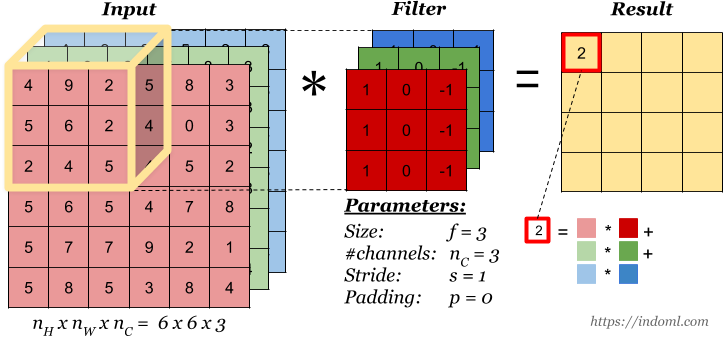
\includegraphics[width=0.75\linewidth]{images/convolutie_rgb.png}
         \captionsetup{font=footnotesize}
         \caption{Convoluții peste volume\cite{conv_rgb}}
\end{figure}

\subsection{Structura unei rețele convoluționale}

Straturile dintr-o rețea convoluțională pot fi împărțite în 3 mari categorii:

\begin{itemize}
    \item \textbf{Straturi convoluționale}
    \item \textbf{Straturi de pooling}
    \item \textbf{Straturi fully connected}
\end{itemize}

\textbf{Straturile convoluționale}

Un \textbf{start convoluțional} este format din filtre și funcții de activare, discutate în capitolul \ref{ch:Gradient Descent}, la care se adaugă paremtri pentru stride și padding. La cei doi parametri se adaugă și bias-ul prezentat în capitolul \ref{ch: Perceptron}. Acesta se adaugă la rezultatul operației de convoluție, pentru fiecare canal de culoare, modificând fromula \ref{eq: rgb_conv}: 

\begin{equation}
    (I * K)(x, y) = \sum_{i=-m}^{m} \sum_{j=-n}^{n} I(x+i, y+j) \cdot K(i, j) + b
\end{equation}

După calcularea hărților de trăsături, fiecare element din hărțile respective este trecut printr-o funcție de activare discutate în capitolul \ref{ch:Gradient Descent}. Rezultatul poartă denumirea de \textbf{hartă de activare}. 

\textbf{Straturile de pooling}

Straturile de pooling sunt folosite pentru a reduce dimensiunea spațială a hărților de activare și au un rol important în a previne \textbf{overfitting-ul}.  Cele mai întâlnite tipuri de pooling sunt \textbf{Max Pooling} și \textbf{Average Pooling}. Max pooling-ul presupune alegerea pixelului cu valorea maximă dintr-o fereastră de dimensiune $n\times n$, în timp ce average pooling folosește toate valorile pentru a calcula valoarea medie ale acestora. Pentru un filtru de dimensiune $2\times 2$: 

\begin{itemize}
    \item \textbf{Max Pooling}:
        \begin{equation}
            P(x, y) = \max \{ I(x, y), I(x+1, y), I(x, y+1), I(x+1, y+1) \}
        \end{equation}
    \item \textbf{Average Pooling}
        \begin{equation}
            P(x, y) = \frac{1}{n^2} \sum_{i=0}^{n-1} \sum_{j=0}^{n-1} I(x+i, y+j)
        \end{equation}
    
\end{itemize}
\newpage
\begin{figure}[h]
         \centering 
         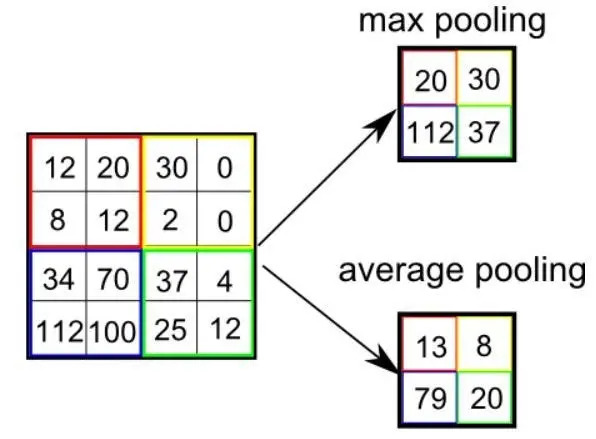
\includegraphics[width=0.55\linewidth]{images/pooling.jpg}
         \captionsetup{font=footnotesize}
         \caption{Max pooling și average pooling\cite{pooling}}
\end{figure}

\textbf{Straturile fully connected}

Numite și straturi dense, sunt folosite spre finalul unei arhitecturi convoluționale. Acestea aplatizează hărțile de activare primtie ca input, într-un vector unidimensional. Practic dupa trecerea prin straturile convoluționale și cele de pooling, output-ul rezultat este dat ca input unei rețele de tip MLP, ce conține straturi fully connected. Ultimul strat al acestei rețele este folosit pentru a face predicțiile.

\begin{figure}[ht]
         \centering 
         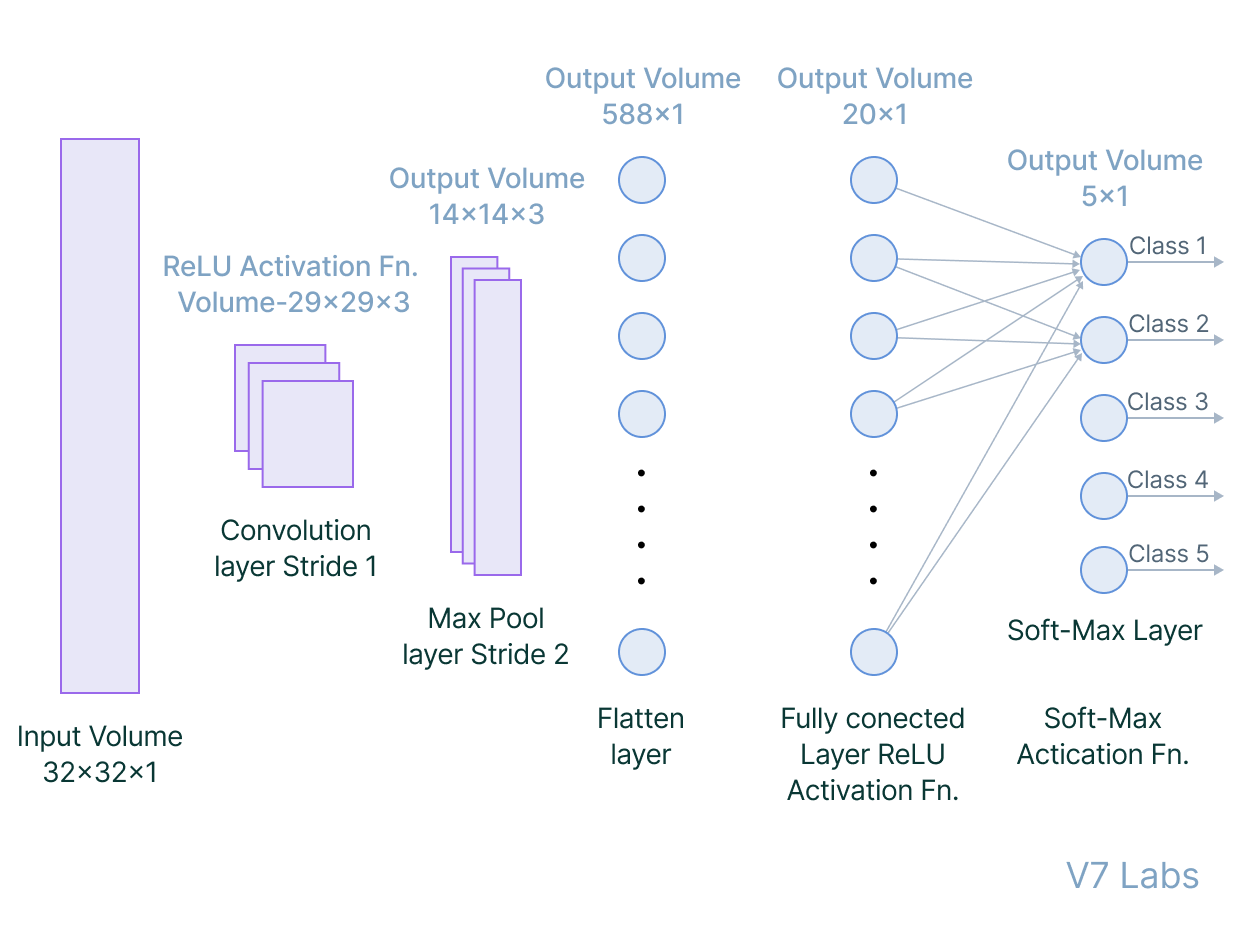
\includegraphics[width=0.65\linewidth]{images/Fully connected.png}
         \captionsetup{font=footnotesize}
         \caption{Structura unei rețele convoluționale\cite{fully-connected}}
\end{figure}

\section{Rețele Generative Adversariale}

